\chapter{Interpreting docking results: docking solution ensemble clustering}

In this chapter we describe why the conduction of a meaningful docking study
requires proper creation and analysis of an ensemble of docking solutions and
explain why clustering is an essential step for making reasonable predictions
about where and how a ligand binds to its receptor. This topic is unfortunately
not well discussed in current molecular docking literature, and existing
technical implementations for the clustering of docking solutions often do not
fit the scientific question and therefore may produce misleading results. Here,
we present a method optimized for clustering docking solution ensembles of GAG
molecules.

\section{Relevance of docking solution clustering}

In the framework of this thesis the term \enquote{docking solution} shall be
understood as a set of ligand atom coordinates, i.e.\ the spatial arrangement of
ligand atoms in the reference coordinate system as defined by the receptor
molecule. As a result of the statistical nature of the docking problem and the
use of pseudo random numbers in implementations of common docking search
algorithms, independent runs of the same docking method are expected to produce
different docking solutions. That is why for seeing the full picture, a
molecular docking method should be applied repetitively, resulting in an
ensemble of docking solutions.

The spatial distribution of docking solutions in that ensemble is governed by a
certain previously unknown probability distribution, which itself is implicitly
determined by the molecular interaction model and search algorithm implemented
in the docking method. Given that we trust the molecular interaction model, the
ultimate goal of a docking study is to obtain the global maximum (and/or some
local maxima) of the named probability distribution. Concept-wise, this is
equivalent to searching the state with highest probability, i.e. lowest energy.
Obtaining local maxima requires complete sampling of that unknown probability
distribution. That is why a docking method must be repeated until convergence
in the spatial distribution of the docking solutions is achieved. Only then the
ensemble reproduces the previously unknown probability distribution and reflects
the molecular interaction model as implemented by the docking method.

If convergence is observed, the next step is to identify the local maxima in the
spatial probability distribution of docking solutions. This problem can be
reformulated in terms of density, i.e.\ as finding the densest agglomerations of
docking solutions in the ensemble. However, a simple evaluation of the
distribution of atoms or molecules per volume would not provide useful results,
because a ligand molecule is comprised of multiple different atoms and has
various asymmetries with respect to shape and property. Spoken freely, the task
is to find agglomerations of docking solutions that are highly \textit{similar}
to each other. Hence, a promising approach is to evaluate the density in terms
of the \textit{similarity} between any two given docking solutions in the
ensemble, subject to the condition that a meaningful molecular similarity
measure can be found. In an abstract sense, the task is to identify groups of
highly similar docking solutions and to separate them from the bulk. This task
fits the general description of \textit{data clustering} as found in
\cite{tan_data_mining}:

\begin{adjustwidth}{1.5cm}{1.5cm}
\textit{\enquote{
The goal is that the objects within a group be similar to one another and
different from the objects in other groups. The greater the similarity (or
homogeneity) within a group and the greater the difference between groups, the
better or more distinct the clustering.}}
\end{adjustwidth}

In conclusion, the most probable ligand molecule placement as predicted by a
certain docking method can be found by \textit{meaningful} clustering of the
converged ensemble of docking solutions. Meaningful clustering can be achieved
by selecting a problem-adjusted clustering method, whereas any data clustering
method has only two major components:

\begin{itemize}
\item the \textit{distance metric}, quantifying the similarity between any two
given objects.
\item a \textit{clustering algorithm}, classifying the objects into groups
(clusters), based on their mutual similarity (i.e.\ distance).
\end{itemize}

It is important to appreciate that both components must be adjusted to the
scientific question, otherwise the result of docking solution clustering might
be meaningless and/or incomparable to other docking studies. Within the next
sections, we introduce a distance metric optimized for GAG molecules and
describe a clustering algorithm appropriate for clustering molecular structure
ensembles in general.


\section{A meaningful distance metric for GAG molecules: RMSatd}

As stated above, spatial clustering evaluates distances between data points
rather than data points themselves. No other information is available to the
clustering algorithm, so the distance metric alone must properly reflect the
similarity between two molecular structures, whereas a large similarity
obviously must correspond to a small distance.

The established way for measuring a structural distance between two molecules
that have an equivalent atomic configuration but different atomic coordinates is
to calculate the root mean square distance ($RMSd$) while pairing up atoms of
same identity:

\begin{equation}
RMSd = \sqrt{\frac{1}{N}\sum{{d_i}^2}}
\end{equation}

Here, each of the $N$ atoms has its own identity and is unambiguously defined by
a unique identifier $i$. $d_i$ is the euclidean distance between two atoms of
the same identity, one in the first structure and the other in the second
structure. This classical $RMSd$ distance metric is for example used in
AutoDockTools \cite{autodock4_adt_2009} for docking solution clustering.

\begin{figure}
\centering
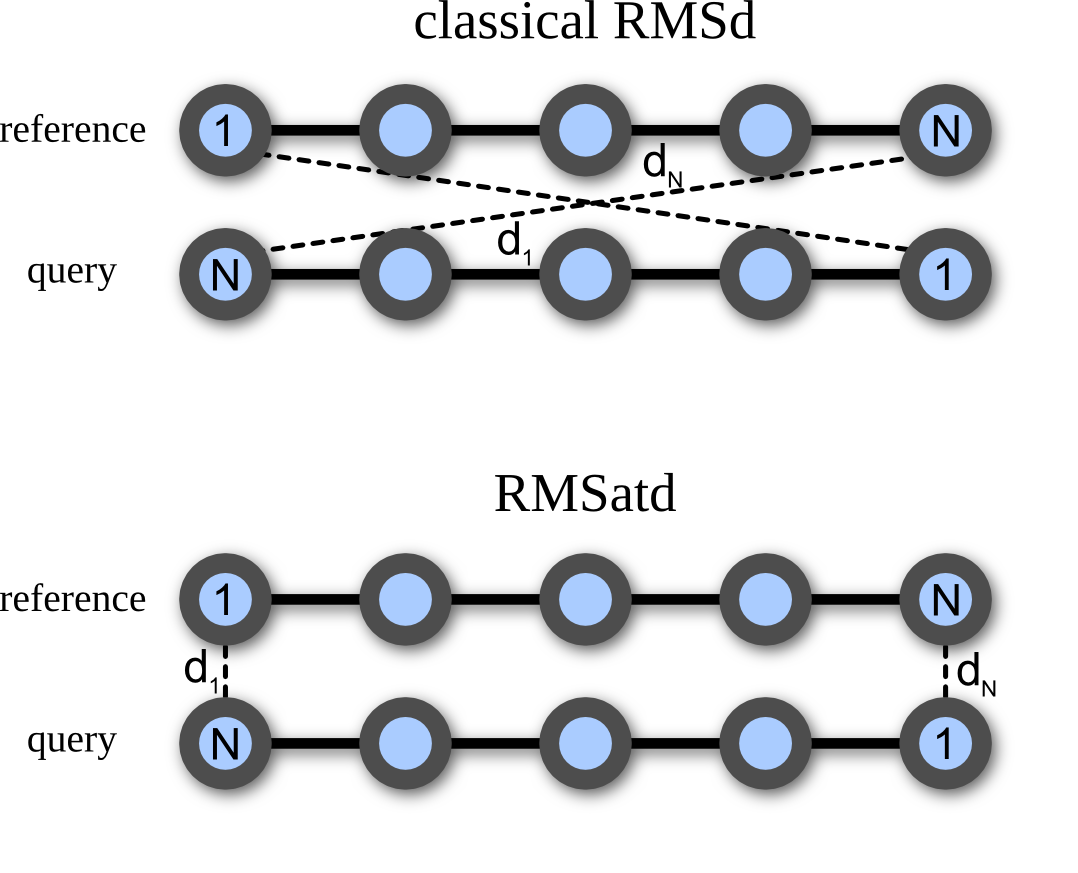
\includegraphics[width=0.7\textwidth]{gfx/clust/RMSd_vs_RMSatd_scheme_03.png}
\caption[]{
Schematic comparison of identity-based atom matching (classical $RMSd$)
\textit{vs.} type-based atom matching ($RMSatd$) by means of an extreme case,
where a linear molecule is compared to itself, after slight vertical shifting
and end-to-end inversion. All atoms (blue) are of the same type. Thick lines
indicate atomic bonds, $1 \dots N$ indicate atom identity. Dashed lines and
$d_i$ indicate pairwise distances used for building the $RMSd$ / $RMSatd$. Top
($RMSd$): atoms of same identity are paired up. Bottom ($RMSatd$): spatially
closest atoms of the same type are paired up.
}
\label{fig:clust:rmsd_vs_rmsatd}
\end{figure}

While the comparison by atom identity makes sense for large molecules such as
proteins, in more simple cases the classical $RMSd$ distance metric might not
properly reflect molecular similarity. This shall be demonstrated by means of an
extreme case, as indicated in the top panel of
\cref{fig:clust:rmsd_vs_rmsatd}. There, a molecule is comprised of linearly
chained atoms of the same type. That molecule exhibits a 2-fold rotational
symmetry: the atomic properties are invariant under the corresponding symmetry
operation (rotation by \SI{180}{\degree}, i.e.\ reversed directionality).
Although the two molecules are positioned almost equivalently, the classical
$RMSd$ measures quite a large distance, i.e.\ low similarity. Assuming bond
lengths and a vertical displacement between both molecules of \SI{1}{\angstrom},
the classical $RMSd$ in that situation would be \SI{3}{\angstrom}.

We propose what we call the root mean square \textit{atom type} distance
$RMSatd$, which works just as the classical $RMSd$, but pairs up spatially
closest atoms of the same type (\cref{fig:clust:rmsd_vs_rmsatd}, bottom panel).
In case of the example situation discussed above, the $RMSatd$ would be
\SI{1}{\angstrom}, i.e.\ more realistically reflects the actual distance between
both molecules than the classical $RMSd$. While GAGs do not have a strict 2-fold
rotational symmetry, they are still highly similar when just reversed along
their end-to-end direction. As demonstrated, this effect is accounted for by the
$RMSatd$ metric. Furthermore, GAGs usually are modeled as strictly periodic
molecules. The $RMSatd$ accounts for this periodicity and considers two GAGs
shifted by $n$ periodic units as structurally similar, while classical $RMSd$
with identity-based matching ignores this characteristic.

Overall, in many cases the $RMSatd$ yields a more intuitive and larger
structural similarity than the classical $RMSd$ metric would. In practice, this
is especially relevant when two GAG structures are slightly displaced relative
to each other along the direction of their longest extent or when comparing two
GAGs with inverted end-to-end directions. On the other hand, for larger
distances between two molecules, the $RMSatd$ converges towards the classical
$RMSd$.


\section{Algorithm of choice: DBSCAN}

One of the of the most popular classes of clustering algorithms is called
\textit{hierarchical clustering}, which is also used for docking solution
clustering in AutoDockTools \cite{autodock4_adt_2009}. Hierarchical clustering
creates a tree-like nested set of groups, i.e.\ a hierarchical grouping, whereas
the actual inter-object distance is evaluated only for the leaf nodes of the
tree. Beyond that, the distance between nodes (groups / clusters) becomes
decisive: calculation of the proximity between two clusters is the key operation
in hierarchical clustering. Obviously, there are various ways to define this
inter-group distance, and it is difficult to come up with one that has an
intuitive meaning with respect to molecular structures. In consequence,
selecting a method for measuring inter- group distance as well as choosing an
inter-group distance cutoff value required for obtaining a definite set of
clusters adds unnecessary complexity for the creation of clusters. During
interpretation of a molecular structure clustering result, we are usually not
interested in the hierarchy at all (while for certain other data types the
hierarchy information for sure is essential).

Clustering algorithms can generally be classified as either
\textit{hierarchical} or \textit{partitional}, whereas partitional clustering
simply is the division of all data objects into non-overlapping subsets, the
clusters \cite{tan_data_mining}. As of the reasoning in the paragraph above, a
molecular structure clustering should in our opinion be from the class of the
partitional clustering algorithms. Conceptually, clustering algorithms can
further be classified as either \textit{complete} or \textit{partial}. In a
complete clustering, each data object is guaranteed to be assigned to one
cluster. Partial clustering on the other hand accounts for a situation where not
all objects in a data set belong to well-defined groups. Those objects that are
not assigned to any cluster usually represent noise, outliers or
\enquote{uninteresting background} \cite{tan_data_mining}.

Clustering aims to find a useful grouping of objects, whereas the common
challenge shared by all kinds of clustering analyses is that
\enquote{usefulness} is defined by the type of data and the goals of the
analysis, and that there is no correct or incorrect approach. Here, the question
we need to answer is:


\begin{adjustwidth}{1.5cm}{1.5cm}
\textit{What are the characteristics of a useful grouping of
molecular structures in a docking solution ensemble?}
\end{adjustwidth}

In order to answer this question, it is helpful to know what different types of
clusters are often observed in real-world data. \cite{tan_data_mining} attempts
to generically describe a few common scenarios. Here, it becomes clear that our
task best fits a density-based clustering, rather than a well-separated,
prototype-based, graph-based or shared-property clustering. Generally spoken, in
\textit{density-based} clustering a cluster is a dense region of objects that is
surrounded by a region of low density.



whereas it becomes clear that
and is Cluster definition


is essential for data
interpretation, Hierarchy information is not and interpretation of a set of
clusters.

is a non-intuitive numerical value that





groups\textit{hierarchical

\lipsum[1-2]

 As for the
clustering algorithm, we implemented DBSCAN \cite{dbscan_ester1996}. It distinguishes
regions of high density from noise which fits the problem of evaluating docking
solution ensembles very well.



The described methodology is implemented and
provided as standard software.

From literature, I identified the DBSCAN algorithm \cite{dbscan_ester1996} to be
appropriate for clustering molecular structures. In contrast to the otherwise
well-established hierarchical clustering, it does not depend on an arbitrarily
defined inter-cluster distance.

At the time of developing the method, according to literature, we were the first
ones implementing DBSCAN for clustering molecular structures. In the meantime,
DBSCAN has also been implemented in cpptraj, a general purpose tool for
analyzing molecular dynamics trajectories.

\subsection{Clustering method overview}

Compared to standard clustering methods, these ingredients significantly
increase the interpretability of GAG docking results and enhance their
comparability. I implemented DBSCAN as well as the optimized distance metric
using linear algebra methods and multi-core software technology. The improved
approach has become standard procedure in the Pisabarro research group and was
used in published work \cite{franz_cathepsin_2013}.


    - Clustering methods overview
        hierarchical clustering implemented in AutoDockTools
            badly implemented, due to $N^2$ dependence very long runtimes
        other methods, quick
        DBSCAN, explain why it makes sense for molecular structures
        cite cpptraj, which also started implementing it

\subsection{DBSCAN parameter optimization}

    - change criteria from eps/minp to N clusters / members
    - reproducibility!
    - comparability among studies
    - characterization of a cluster via eps


\section{Clustering method implementation}

\subsection{Efficient implementation of DBSCAN for numpy}

        - Custom implementation of the DBSCAN algorithm

\subsection{Efficient implementation of RMSatd for numpy}

        - Custom implementation of the DBSCAN algorithm
        - examples
            http://scikit-learn.org/stable/modules/clustering.html
            http://bit.ly/1pKNv7v


\subsection{Parameter optimization}

        - brute force plus local optimization

\subsection{Architecture of cluster-pdb-structures}

            command line tool, simple PDB parser files
            distance matrix calculation on multiple cores via Unix fork()

            input: structure ensemble, DBSCANopt parameters
            output: structure files, stat summary


            open source at bitbucket..


\textbf{
This problem-oriented approach significantly increases the
interpretability of GAG docking results and enhances their comparability. By
now, this methodology is applied in the context of several projects in the
Pisabarro research group.
}



